\section{Execution}
\label{sec:Durchführung}

\subsection{Setup}
The Setup consits of a Diodelaser, two Detectors, a camera, an Absorption Cell, a neutral density filter, an Oszilloscop, an Infrared Card and a Controller for the Laser.
The Diodelaser has a wavelength of about $\lambda = \SI{785}{\nano\meter}$.
The Absorption cell consits of a glass chamber that is filled with Rubidium vapor, that is used for its Flourescence effect while absorbing the laser light.
The Oszilloscop will help to monitor the Absorption of the laser light through deteing the light intensity with the Detectors which are connected to the Oszilloscop.
The Infrared card helps to find the laser beam beacause it is not visible for the naked eye.
The Controller is the main power source for all the devices in the Experiment and a way to controlle the configuartion of the components

\subsubsection{Lasing}
First the laser is being conected to the controller so that it is possible to controlle the laser current and temperature.
Usually the lasers temperature and the Top knob configuartion of the laser has to be fine tuned before the Experiment, but this was not the case for us because the configuartion were already good from the begining on.
After the alingment the infrared card is placed infront of the laser, and the camera is faced towards the card.
The camera gets connected to the power supply.
Now the laser current is switched on but it is being kept at a low voltage.
A picture is taken from the dot thats visible on the infrared card, while the laser current is low.
The current is being increased gradually until the brightness of the red dot on the infrared card suddenly increases heavily and a speckle pattern is visible around the dot.
This is the laser threshold of which also a picture is being taken.

\subsubsection{Setting up the Rubidium Flourescence}
For this step the Infrared card gets removed and switch out by the Absorption cell.
The laser beam should pass trough the center of the cell.
To observe the Flourescence of the Rubidium vapor the camera is pointed into the cell.
The piezo controller input gets connected to the ramp generator and its output to the Oszilloscop channel 1.
The other ramp generator output goes to the Oszilloscop trigger.
Now the generator frequenzy is set to $\SI{10}{\Hz}$, the attenuator knob of the piezo is set to 1 and the amplitude of the ramp generator is set to 10.
With the DC Offset knob a large-amplitude triangle is produced on the Oszilloscop.
Now the Laser current gets tweaked until flourescence is visible in the chamber.
If no flourescence is visible the Side knob of the laser has to be adjusted until it starts.
If flourescence is visible the setting of the Side knob has to be changed until the flourescence is at a maximum.

\subsubsection{Observing the Spectrum of Absorption}
To observe the Spectrum the Photodiode Detectors need to be connected to the Powersupply located at the controller.
The output of one of the Detectors gets connected to the Oszilloscop channel 2.
Now the Detector thats connected to the Oszilloscop should be placed in a way that it intercepts the beam, comming out of the absorption cell.
The Photodiode Detector has to be moved around a bit so it really measures the full intensity of the beam.
To prevent the Detector from moving it should be bolted down, after it is aligned.
Also the room lights should be switched off.
\\\\
The next step is to place the neutral density filter between the Laser and the absorption cell.
Now a Absorption spectrum should be visible on the Oszilloscop even tough its not optimal, because there can still be mode hops in the laser light.

\subsubsection{Removing mode hops}
Now the Side knob has to be adjusted to produce a clear absorption spectrum.
For this an alled wrench is used to make very small adjustments to the Side knob.
There should be six to eight modes thorugh which one moves when the allen wrench is turned.
The middle of that mode pattern is the point that should be aimed for.
Now the Laser current and the Piezo DC Level gets tweaked until no mode hops or extra features are visible any more.

\subsubsection{Using two Photodiods to compare the neutral beam and the absorption beam}
A BNC splitter gets added at the ramp generator, this connects to the current modulation input and the piezo controller input.
Now the ramp generator amplitude gets turned up to maximum and the current attenuator knob gets turned until one full Rubidium spectrum is visible.
Now a beam splitter has to be installed infront of the Rubidium chamber.
This splitts the beam $50/50$ and provides a possebility to compare the initial beam with the beam that passed thorugh the chamber.
A Photodiode gets placed infront of the beam that does not pass through the chamber.
This photodiodes output gets connected to the Detector input channel 1 on the controller.
The other photodiodes otuput gets connected to Detector input channel 2 on the controller.
The Monitor output gets connected to input channel 1 of the Oszilloscop.
Input channel 2 of the Oszilloscop is not connected.
The trigger channel of the Oszilloscop gets connected to the sync. output of the ramp generator.
A scetch of the Setup is shown in Figure \ref{fig:setup}.

\begin{figure}
    \centering
    \caption{The setup with two Detectors as a way to compare the initial beam with the beam that passed through the chamber. The pictures is taken from source \cite[16]{anleitung_exp}}
    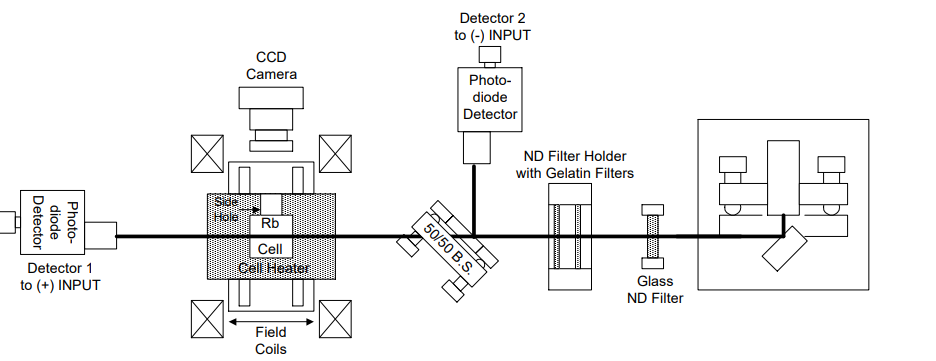
\includegraphics[width=\textwidth]{content/data/setup}
    \label{fig:setup}
\end{figure}

Now the Gain knob of the Detector input should be turned until the signal lies between $2-6 \,\si{\volt}$.
The last step is to turn the balance knobs (+) and (-) until the Oszilloscop shows the Absorption peaks of the Rubidium and a completly level graph anywhere else.
A picture of this graph is taken.
